\newpage
\section{Turn Up the Volume!}

In this activity, we will investigate formulas for area and
volume.


\begin{prob}
Explain how the following picture ``proves'' that the area of a right
  triangle is one half of the base times the height.
\[
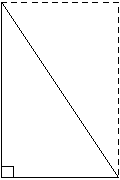
\includegraphics{../graphics/pbpAreaRight.pdf}
\]
\end{prob}


\begin{prob}
Cavalieri's principle states:\index{Cavalieri's principle}
\begin{quote}
Shearing parallel to a fixed direction does not change the
$n$-dimensional measure of an object.
\end{quote}
What is this saying?
\end{prob}




\begin{prob}
Building on the first two problems, explain how the following picture
  ``proves'' that the area of any triangle is one half of the base times the
  height.
\[
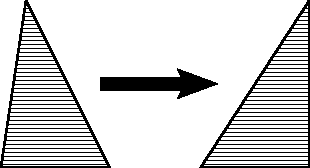
\includegraphics{../graphics/pbpShearTri.pdf}
\]
\end{prob}




\begin{prob}
Give an intuitive argument explaining why Cavalieri's principle is
true.
\end{prob}


\begin{prob}
Explain how to use a picture to ``prove'' that a triangle of a given
  area could have an arbitrarily large perimeter.
\end{prob}



\begin{prob}
Sketch a net for a right pyramid of height $2''$ with a $2'' \times
2''$ square base. Share your sketch with your neighbor---does it look
OK?
\end{prob}


\begin{prob}
Give detailed diagrams that show that a cube can be constructed from
three equal pyramids.
\end{prob}

\begin{prob}
Use your work above to derive a formula for the volume of a
right pyramid with a square base. The formula should be in terms of
the side length of the square base.
\end{prob}

\begin{prob}
Give a formula for \textbf{every} pyramid with an $s\times s$ square base of height $s$ in terms of $s$. 
\end{prob}


